\documentclass{article}
\usepackage[utf8]{inputenc}
\usepackage{amsmath}
\usepackage{utp-doc}
\usepackage{graphicx}
\usepackage{geometry}
\usepackage{xcolor}
\usepackage{tikz}
\usepackage{pifont}


%\title{AVS.01.01.01: Análisis Metrológico de un Vehículo Eléctrico Compacto}
%\author{Profesor [Su Nombre]}
%\date{\today}

\begin{document}
	
	%
	% --- Título de la Lectura ---
	\practicatitle{AVS.02.01.01: Selección de Proveedor Basada en Certificaciones}
	
	% --- Metadatos de la Actividad ---
	\textbf{Asignatura:} Metrología \\
	\textbf{Unidad II:} - Normatividad en Metrología Automotriz 
	
	\vspace{5mm}
	\hrule
	\vspace{5mm}
% \title{AVS.02.01.01: Selección de Proveedor Basada en Certificaciones}
\section*{Introducción}

En la \hl{industria automotriz moderna}, la \hl{selección de proveedores} no se basa únicamente en el precio de los productos, sino también en la \hl{calidad, confiabilidad y cumplimiento normativo} que pueden ofrecer. Las \hl{certificaciones y estándares metrológicos} que posee un proveedor son indicadores clave de su capacidad para entregar productos que cumplan con las \hl{especificaciones técnicas} requeridas.

El presente caso de estudio permite al estudiante \hl{comprender la importancia de las certificaciones} en la cadena de suministro automotriz, \hl{identificar y clasificar diferentes tipos de normas} y \hl{analizar cómo estas influyen} en la toma de decisiones comerciales en un contexto real de la industria.

\section*{Objetivo General}

\hl{Analizar y comparar} las certificaciones metrológicas de diferentes proveedores para \hl{recomendar la mejor opción} de suministro, considerando el \hl{impacto de las normas y estándares} en la calidad del producto final y el cumplimiento de requisitos del cliente.

\section*{Actividad Previa al Desarrollo del Caso}

Antes de desarrollar el caso de estudio, revisa el \hl{material teórico} proporcionado y contesta el siguiente \hl{cuestionario}. Esto te ayudará a contextualizar los conceptos y a aprovechar mejor el análisis del caso.

\begin{enumerate}
    \item \textbf{¿Qué es una certificación y por qué es importante en la industria automotriz?}
    \item \textbf{¿Cuál es la diferencia entre una norma obligatoria y una norma voluntaria?}
    \item \textbf{Menciona 3 organismos que emiten normas para la industria automotriz.}
    \item \textbf{¿Qué significa que un proveedor tenga certificación ISO 9001?}
    \item \textbf{¿Por qué es importante que los instrumentos de medición estén calibrados?}
\end{enumerate}

\section*{Descripción del Caso de Estudio}

\subsection*{Escenario}

\hl{``Motores del Norte S.A.''} es una empresa mexicana que ensambla motores para automóviles compactos. La empresa ha crecido significativamente y ahora necesita seleccionar un nuevo proveedor para \hl{juntas de culata}, un componente crítico que debe cumplir tolerancias de medición muy estrictas.

\subsection*{Situación}

El Departamento de Compras ha recibido \hl{tres propuestas} de diferentes proveedores para el suministro de \hl{10,000 juntas de culata} mensuales durante los próximos 2 años. Todos los proveedores ofrecen productos técnicamente similares y precios competitivos, pero tienen \hl{diferentes niveles de certificación} y cumplimiento normativo.

\begin{figure}[h!]
    \centering
    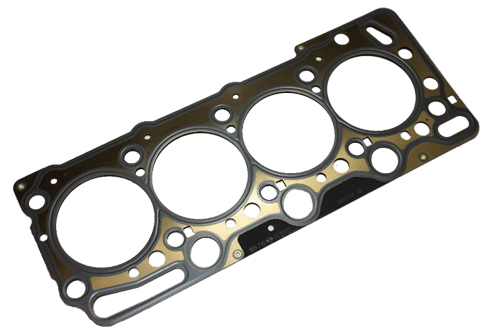
\includegraphics[width=0.6\textwidth]{junta-de-culata.png}
    \caption{Ejemplo de una junta de culata de motor.}
    \label{fig:junta_culata}
\end{figure}

\subsection*{Requerimientos Técnicos}
\begin{itemize}
    \item Tolerancia dimensional: $\pm$0.05 mm en espesor
    \item Material: Grafito compuesto con resistencia térmica hasta 250°C
    \item Presión de trabajo: Hasta 15 bar
    \item Cumplimiento: Con normas mexicanas para vehículos
\end{itemize}

\subsection*{Información de los Proveedores}

\subsubsection*{Proveedor A: "TecnoPartes Guadalajara"}
\begin{itemize}
    \item Ubicación: Guadalajara, Jalisco, México
    \item Experiencia: 8 años en el mercado
    \item Precio ofertado: \$45.00 MXN por pieza
    \item Certificaciones actuales:
    \begin{itemize}
        \item Sin certificación ISO formal
        \item Registro ante PROFECO como fabricante
        \item Cumple con NOM-012-SCT-2-2017 (Pesos y dimensiones)
    \end{itemize}
    \item Sistema de medición:
    \begin{itemize}
        \item Calibradores básicos sin certificado de calibración
        \item Mediciones realizadas por operadores de producción
        \item Registros manuales de control de calidad
        \item Sin trazabilidad metrológica documentada
    \end{itemize}
    \item Información adicional:
    \begin{itemize}
        \item Empresa familiar en crecimiento
        \item Tiempo de entrega: 15 días
        \item Garantía: 6 meses por defectos de fabricación
        \item Referencias: 2 clientes pequeños en el mercado nacional
    \end{itemize}
\end{itemize}

\subsubsection*{Proveedor B: "Componentes Industriales de México"}
\begin{itemize}
    \item Ubicación: Tijuana, Baja California, México
    \item Experiencia: 15 años en el mercado
    \item Precio ofertado: \$52.00 MXN por pieza
    \item Certificaciones actuales:
    \begin{itemize}
        \item ISO 9001:2015 (Sistema de Gestión de Calidad)
        \item Certificación IATF 16949:2016 (Estándar automotriz)
        \item Registro EMA para laboratorio de mediciones
    \end{itemize}
    \item Sistema de medición:
    \begin{itemize}
        \item Instrumentos calibrados por laboratorio acreditado EMA
        \item Personal capacitado en técnicas de medición
        \item Sistema digital de registro de mediciones
        \item Trazabilidad metrológica hasta CENAM
    \end{itemize}
    \item Información adicional:
    \begin{itemize}
        \item Proveedor de GM y Ford México
        \item Tiempo de entrega: 10 días
        \item Garantía: 2 años por defectos de fabricación
        \item Auditorías de calidad semestrales
    \end{itemize}
\end{itemize}

\subsubsection*{Proveedor C: "Global Auto Components"}
\begin{itemize}
    \item Ubicación: San Luis Potosí, SLP, México
    \item Experiencia: 25 años en el mercado
    \item Precio ofertado: \$58.00 MXN por pieza
    \item Certificaciones actuales:
    \begin{itemize}
        \item ISO 9001:2015 (Sistema de Gestión de Calidad)
        \item IATF 16949:2016 (Estándar automotriz)
        \item ISO 14001:2015 (Gestión Ambiental)
        \item Certificación Six Sigma Black Belt
        \item Acreditación ISO 17025 para su laboratorio interno
    \end{itemize}
    \item Sistema de medición:
    \begin{itemize}
        \item Laboratorio interno con patrones certificados
        \item CMM (Máquina de Medición por Coordenadas)
        \item Personal certificado en metrología dimensional
        \item Sistema automatizado de control estadístico de procesos
    \end{itemize}
    \item Información adicional:
    \begin{itemize}
        \item Proveedor Tier 1 para BMW, Audi y Mercedes-Benz
        \item Tiempo de entrega: 7 días
        \item Garantía: 3 años por defectos de fabricación
        \item Exporta a 12 países
    \end{itemize}
\end{itemize}

\section*{Desarrollo del Caso de Estudio}

\subsection*{Fase 1: Identificación y Clasificación de Normas (25 puntos)}

\subsubsection*{1.1 Inventario de Certificaciones}

Para cada proveedor, identifica y clasifica sus certificaciones:
\begin{enumerate}
    \item \textbf{Elabora una tabla} con todas las certificaciones mencionadas
    \item \textbf{Investiga qué significa} cada certificación (máximo 3 renglones por certificación)
    \item \textbf{Clasifica cada certificación} según:
    \begin{itemize}
        \item Tipo: Obligatoria o Voluntaria
        \item Alcance: Nacional, Internacional o Sectorial
        \item Área: Calidad, Ambiental, Metrológica, Automotriz
    \end{itemize}
\end{enumerate}

\subsubsection*{1.2 Análisis de Organismos Emisores}

Investiga y presenta información básica sobre:
\begin{enumerate}
    \item \textbf{¿Qué es ISO} y por qué sus normas son importantes?
    \item \textbf{¿Qué es IATF} y su relación con la industria automotriz?
    \item \textbf{¿Qué es CENAM} y su función en México?
    \item \textbf{¿Qué es EMA} y para qué sirve su acreditación?
\end{enumerate}

\subsection*{Fase 2: Análisis Comparativo de Proveedores (30 puntos)}

\subsubsection*{2.1 Matriz de Comparación}

Crea una matriz comparativa que incluya:
\begin{enumerate}
    %\item \textbf{Certificaciones por proveedor} (usar \texttt{\checkmark} o \texttt{\ding{55}})
    \item \textbf{Nivel de cumplimiento normativo} (Alto, Medio, Bajo)
    \item \textbf{Confiabilidad del sistema de medición} (Alta, Media, Baja)
    \item \textbf{Trazabilidad metrológica} (Sí/No/Parcial)
\end{enumerate}

\subsubsection*{2.2 Análisis de Ventajas y Desventajas}

Para cada proveedor, identifica:
\begin{enumerate}
    \item \textbf{3 ventajas principales} derivadas de sus certificaciones
    \item \textbf{3 desventajas o riesgos} por falta de certificaciones
    \item \textbf{Impacto en la calidad} del producto final
    \item \textbf{Confiabilidad a largo plazo} como proveedor
\end{enumerate}

\subsubsection*{2.3 Evaluación de Sistemas de Medición}

Compara los sistemas de medición:
\begin{enumerate}
    \item \textbf{Nivel de equipamiento} de cada proveedor
    \item \textbf{Competencia del personal} en mediciones
    \item \textbf{Confiabilidad de los resultados} de medición
    \item \textbf{Capacidad de mejora continua}
\end{enumerate}

\subsection*{Fase 3: Análisis de Riesgos y Beneficios (20 puntos)}

\subsubsection*{3.1 Identificación de Riesgos}

Por cada proveedor, identifica riesgos potenciales:
\begin{enumerate}
    \item \textbf{Riesgos de calidad:}
    \begin{itemize}
        \item Productos fuera de especificación
        \item Variabilidad en las mediciones
        \item Falta de control de procesos
    \end{itemize}
    \item \textbf{Riesgos comerciales:}
    \begin{itemize}
        \item Pérdida de clientes por mala calidad
        \item Costos de garantía y devoluciones
        \item Daño a la reputación de la empresa
    \end{itemize}
    \item \textbf{Riesgos legales:}
    \begin{itemize}
        \item Incumplimiento de normas obligatorias
        \item Responsabilidad por productos defectuosos
        \item Sanciones de autoridades
    \end{itemize}
\end{enumerate}

\subsubsection*{3.2 Análisis de Beneficios}

Identifica beneficios de elegir proveedores certificados:
\begin{enumerate}
    \item \textbf{Beneficios técnicos:}
    \begin{itemize}
        \item Mayor confiabilidad en las mediciones
        \item Productos consistentes con especificaciones
        \item Mejora continua de procesos
    \end{itemize}
    \item \textbf{Beneficios comerciales:}
    \begin{itemize}
        \item Acceso a mercados internacionales
        \item Reconocimiento de clientes exigentes
        \item Ventaja competitiva
    \end{itemize}
\end{enumerate}

\subsection*{Fase 4: Evaluación Integral y Recomendación (15 puntos)}

\subsubsection*{4.1 Análisis Costo-Beneficio Simplificado}

Realiza un análisis básico considerando:
\begin{enumerate}
    \item \textbf{Costo inicial} por pieza de cada proveedor
    \item \textbf{Costos ocultos} potenciales:
    \begin{itemize}
        \item Re-trabajos por mala calidad
        \item Inspecciones adicionales
        \item Pérdida de clientes
    \end{itemize}
    \item \textbf{Beneficios cuantificables:}
    \begin{itemize}
        \item Reducción de rechazos
        \item Menor tiempo de inspección
        \item Mayor satisfacción del cliente
    \end{itemize}
\end{enumerate}

\subsubsection*{4.2 Matriz de Decisión}

Crea una matriz de decisión con los siguientes criterios:

\begin{tabular}{|l|c|c|c|c|}
\hline
\textbf{Criterio} & \textbf{Peso (\%)} & \textbf{Proveedor A} & \textbf{Proveedor B} & \textbf{Proveedor C} \\
\hline
Precio & 20\% & & & \\
Certificaciones & 25\% & & & \\
Sistema de medición & 20\% & & & \\
Experiencia & 15\% & & & \\
Tiempo de entrega & 10\% & & & \\
Garantía & 10\% & & & \\
\hline
\textbf{TOTAL} & \textbf{100\%} & & & \\
\hline
\end{tabular}

\textbf{Escala de calificación:} 1 = Deficiente, 2 = Regular, 3 = Bueno, 4 = Muy bueno, 5 = Excelente

\subsection*{Fase 5: Recomendación Final (10 puntos)}

\subsubsection*{5.1 Selección del Proveedor}

Basándote en tu análisis, \textbf{recomienda qué proveedor elegir} y justifica tu decisión considerando:
\begin{enumerate}
    \item \textbf{Razón principal} de tu elección
    \item \textbf{Beneficios esperados} de esta decisión
    \item \textbf{Riesgos asumidos} y cómo minimizarlos
    \item \textbf{Impacto a largo plazo} en la empresa
\end{enumerate}

\subsubsection*{5.2 Plan de Acción}

Propone un plan básico de implementación:
\begin{enumerate}
    \item \textbf{Pasos} para iniciar la relación con el proveedor seleccionado
    \item \textbf{Verificaciones} que debe hacer Motores del Norte
    \item \textbf{Seguimiento} del desempeño del proveedor
    \item \textbf{Revisiones} periódicas de la decisión
\end{enumerate}

\section*{Hoja de Trabajo (Sugerida)}

A continuación, se presenta una estructura sugerida para organizar los resultados de su análisis.

\subsection*{Fase 1: Inventario de Certificaciones}

\begin{tabular}{|l|l|l|l|l|l|}
\hline
\textbf{Proveedor} & \textbf{Certificación / Norma} & \textbf{Significado Breve} & \textbf{Tipo} & \textbf{Alcance} & \textbf{Área} \\
\hline
\textbf{A} & & & & & \\
\textbf{B} & & & & & \\
\textbf{C} & & & & & \\
\hline
\end{tabular}

\subsection*{Fase 2: Matriz de Comparación}

\begin{tabular}{|l|c|c|c|}
\hline
\textbf{Criterio} & \textbf{Proveedor A} & \textbf{Proveedor B} & \textbf{Proveedor C} \\
\hline
\textbf{Certificaciones} & & & \\
\textbf{Cumplimiento Normativo} & & & \\
\textbf{Confiabilidad de Medición} & & & \\
\textbf{Trazabilidad Metrológica} & & & \\
\hline
\end{tabular}

\subsection*{Fase 4: Matriz de Decisión}

*Llene la siguiente tabla con su calificación (1-5) y el resultado ponderado.*

\begin{tabular}{|l|c|c|c|c|c|c|c|}
\hline
\textbf{Criterio} & \textbf{Peso (\%)} & \textbf{Calificación A} & \textbf{Pond. A} & \textbf{Calificación B} & \textbf{Pond. B} & \textbf{Calificación C} & \textbf{Pond. C} \\
\hline
Precio & 20\% & & & & & & \\
Certificaciones & 25\% & & & & & & \\
Sistema de medición & 20\% & & & & & & \\
Experiencia & 15\% & & & & & & \\
Tiempo de entrega & 10\% & & & & & & \\
Garantía & 10\% & & & & & & \\
\hline
\textbf{TOTAL} & \textbf{100\%} & & \textbf{-} & & \textbf{-} & & \textbf{-} \\
\hline
\end{tabular}

\subsection*{Fase 5: Recomendación Final}

\textbf{Proveedor Seleccionado:}

\vspace{1cm}

\textbf{Justificación Principal:}

\vspace{3cm}

\section*{Forma de Entrega del Trabajo}

El estudiante deberá entregar un \hl{único archivo en formato PDF} (`.pdf`) que corresponde al reporte técnico del caso de estudio. El documento debe ser claro, ordenado y contener los siguientes elementos:

\subsection*{1. Datos Generales (Portada)}
\begin{itemize}
    \item Nombre completo del estudiante y matrícula.
    \item Asignatura: Metrología.
    \item Nombre de la actividad: `AVS.02.01.01: Selección de Proveedor Basada en Certificaciones`.
    \item Nombre del docente.
    \item Fecha de elaboración.
\end{itemize}

\subsection*{2. Cuestionario Previo}
Respuestas claras y bien fundamentadas a las 5 preguntas de la sección "ACTIVIDAD PREVIA AL DESARROLLO DEL CASO".

\subsection*{3. Desarrollo del Caso de Estudio}
Presentar el análisis de cada fase, utilizando las tablas y matrices de la hoja de trabajo para estructurar la información.

\subsection*{4. Conclusiones y Bibliografía}
\begin{itemize}
    \item \textbf{Conclusiones:} Reflexión personal sobre la importancia de la normatividad en la selección de proveedores (mínimo 5 renglones).
    \item \textbf{Bibliografía:} Incluir al menos dos fuentes de consulta en formato APA.
\end{itemize}

\section*{Recursos de Apoyo}

\begin{itemize}
    \item \textbf{ISO 9001:} Sistema de gestión de calidad
    \item \textbf{IATF 16949:} Estándar específico para industria automotriz
    \item \textbf{ISO 14001:} Sistema de gestión ambiental
    \item \textbf{ISO 17025:} Laboratorios de ensayo y calibración
    \item \textbf{CENAM:} Centro Nacional de Metrología (México)
    \item \textbf{EMA:} Entidad Mexicana de Acreditación
\end{itemize}

\end{document}
